\documentclass[a4paper, 14pt]{article}

\usepackage[english, russian]{babel}
\usepackage[T2A]{fontenc}
\usepackage[utf8]{inputenc}
\usepackage{mathtext}
\usepackage{amsfonts}
\usepackage{ amssymb }
\usepackage{amsmath}
\usepackage{graphics}
\usepackage{graphicx}
\usepackage{wrapfig}
\usepackage{geometry}
\geometry{
	a4paper,
	total={170mm, 257mm},
	left=20mm,
	top=10mm}


\author{Абакшин В.С. Б05-207}
\title{3.3.4. Эффект Холла в полупроводниках.}
\date{\today}
\begin{document}
	\maketitle
	\textbf{Цель работы}: измерение подвижности и концентрации носителей заряда в полупроводниках.
	
	
	\textbf{В работе используются}: электромагнит с источником питания, амперметр, милливеберметр, реостат, источник питания, цифровой вольтметр, образцы легированного германия.\\
	\section*{Описание работы}
	\begin{figure}[h!]
		\centering
		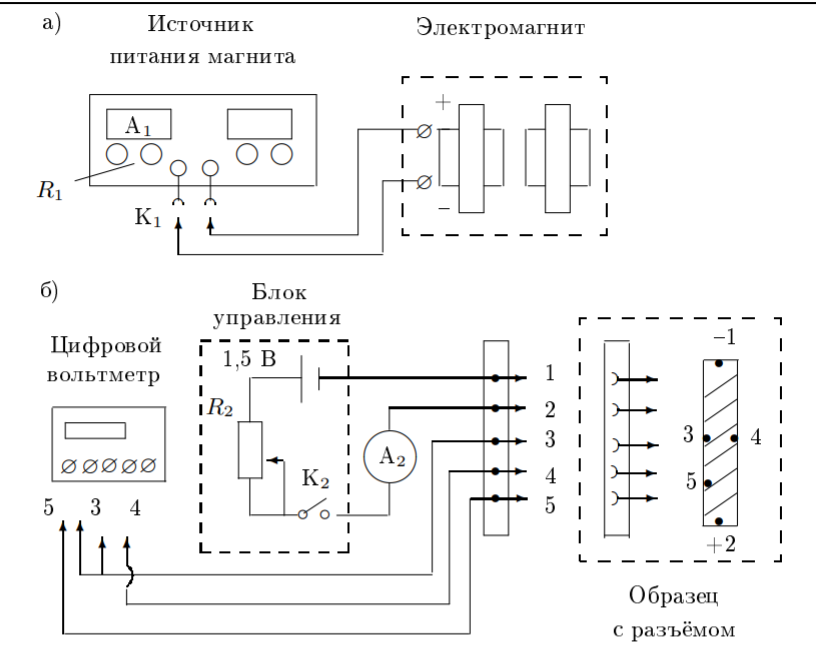
\includegraphics[scale=0.7]{1.png}
		\caption{Схема установки}
	\end{figure}
	Схема для измерения ЭДС Холла представлена на рисунке. В зазоре электромагнита создаётся постоянное магнитное поле, величину которого можно менять регуляторами источника питания электромагнита. Градуировка магнита проводится при помощи милливеберметра.\\
	Образец из легированного германия, смонтированный в специальном держателе, подключается к источнику питания. При замыкании К$_2$ вдоль длинной стороны образца течёт ток, величина которого регулируется реостатом $R$ и измеряется миллиамперметром. В образце, помещённом в зазор, возникает разность потенциалов $U_{34}$, которая измеряется с помощью цифрового вольтметра.
	Влияние омического падения напряжения исключается измерением напряжения $U_0$ между 3 и 4 в отсутствие магнитного поля. По знаку $\mathcal{E} = U_{34} \pm U_0$ можно определить характер проводимости -- электронный или дырочный, зная направление тока в образце и направление магнитного поля.\\
	Померив ток $I_{35}$ в образце и напряжение $U_{35}$ между контактами 3 и 5 в отсутствие магнитного поля можно рассчитать проводимость материала по формуле
	$$
	\sigma = \frac{IL_{35}}{U_{35}al},
	$$
	где $L_{35}$ -- расстояние между контактами 3 и 5, а $a$ и $l$ -- толщина и ширина образца.
	\section*{Ход работы и обработка результатов}
	
	 1) Проградуируем электромагнит. Определим связь между индукцией $B$ магнитного поля в зазоре электромагнита и током $I_M$ через обмотку сняв зависимость потока $\text{Ф} = BSN$, пронизывающего пробную катушку, находящуюся в зазоре, от тока $I_M$. Значение $SN = 72~\text{см}^2 \cdot \text{вит}$.
		\begin{table}[h]
			\centering
			\begin{tabular}{|l|l|l|l|l|l|l|l|l|}
				\hline
				$I$, А  & 0 & 0.27 & 0.54  & 0.81   & 1.08     & 1.35   & 1.58 & $\sigma_I = 0.01$ \\ \hline
				$\Phi$, мВб & 0.12 & 1.8 & 3.7 & 5.2 & 6.5 & 7.3 & 7.9 &$\sigma_{\Phi} = 0.05$ \\ \hline
				$B$, Тл & 0.02 & 0.25 & 0.51 & 0.72 & 0.90 & 1.01 & 1.10 & $\sigma_B = 0.007$ \\ \hline
			\end{tabular}
			\caption{Измерение магнитной индукции при различных значениях $I_{\text{магн}}$ (градуировка)}
		\end{table}
	Построим график зависимости $B = f(I)$:
	
	\begin{figure}[h]
		\centering
		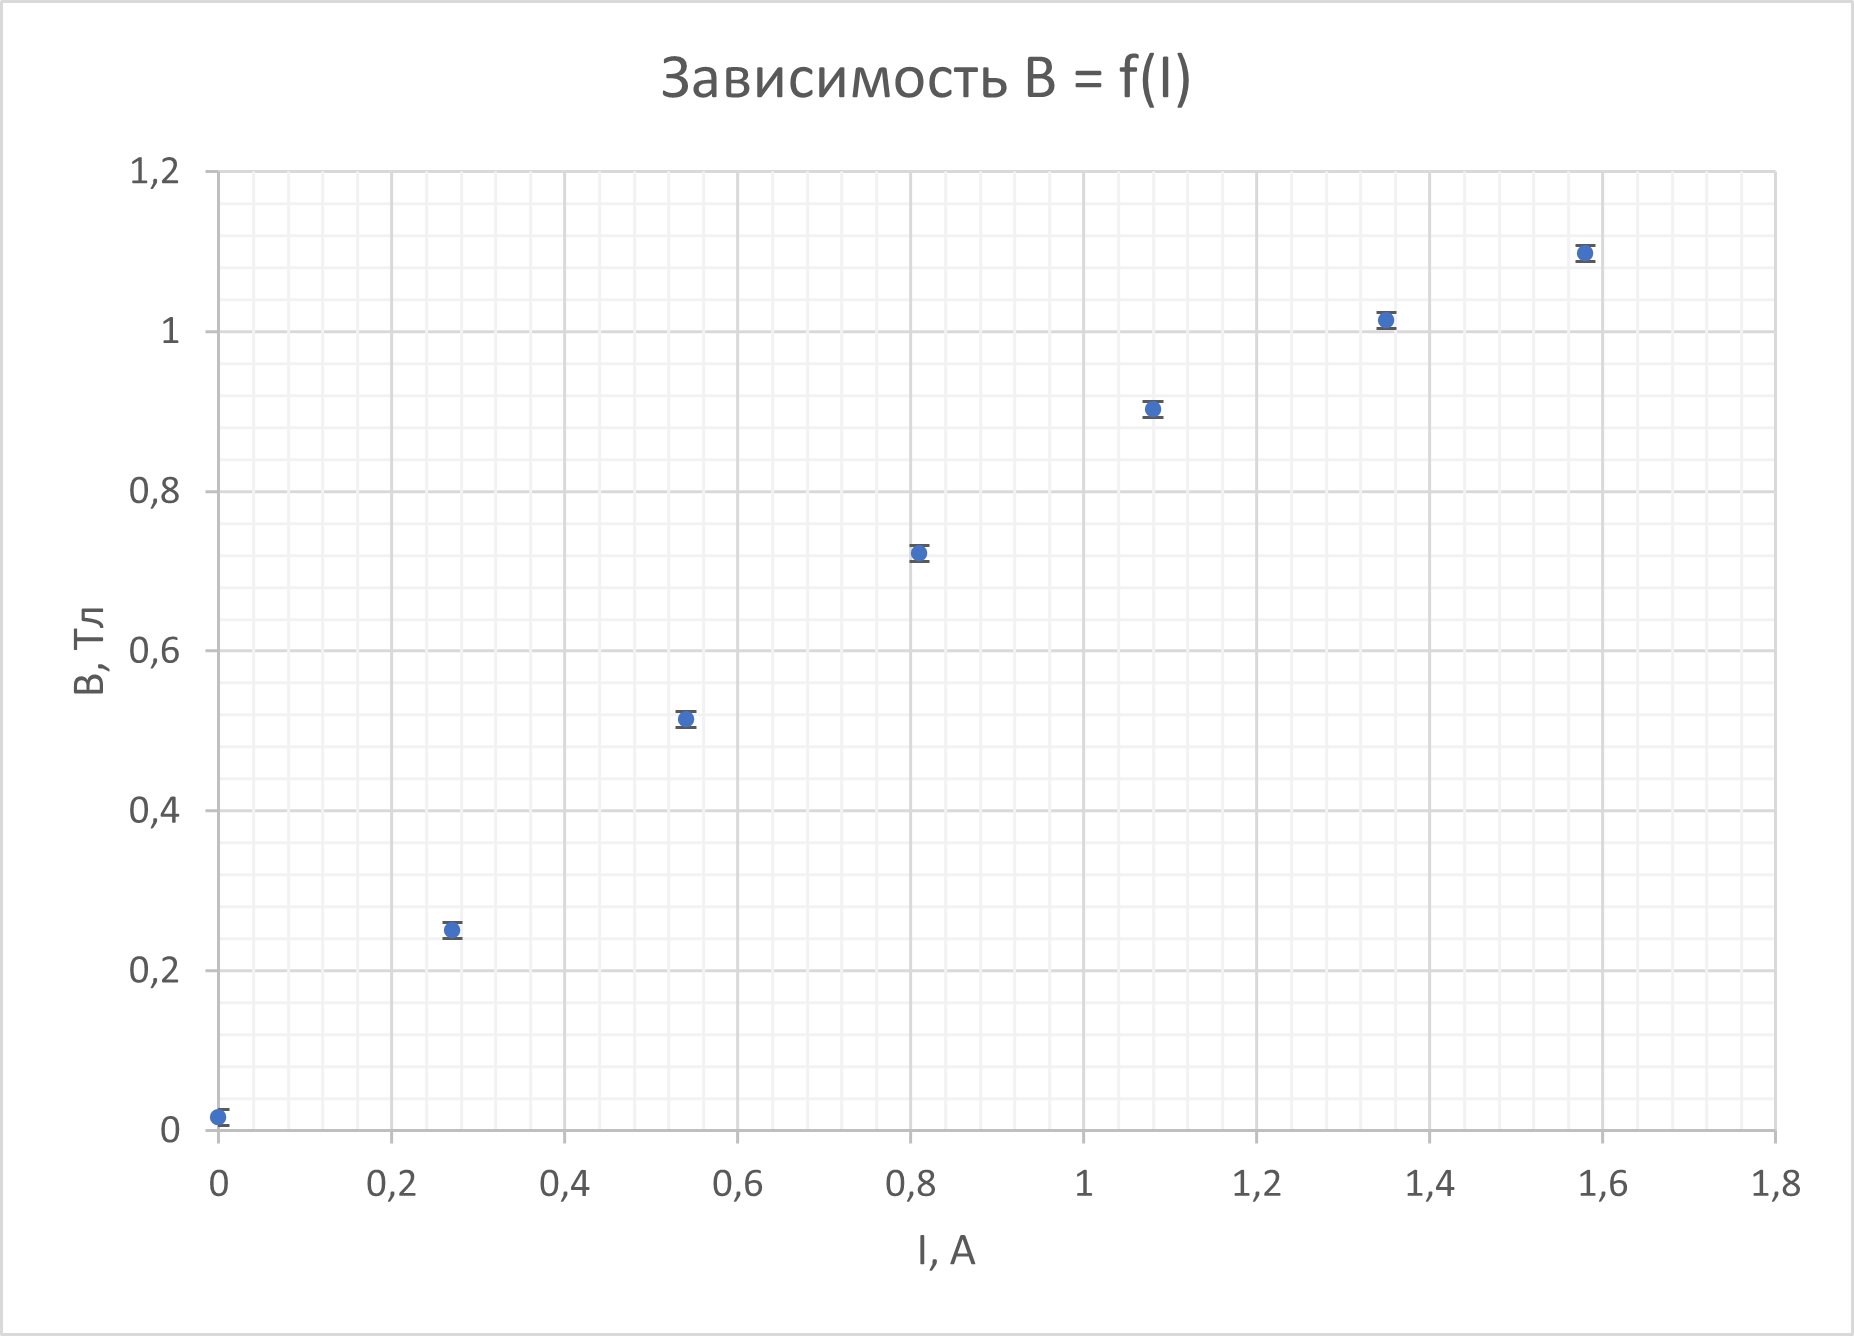
\includegraphics[scale = 1.05]{Gr1}
		\caption{Зависимость $B = f(I)$}
	\end{figure}
	
	2) Проведём измерение ЭДС Холла. Для этого вставим образец в зазор выключенного электромагнита и определим $U_0$ между контактами 3 и 4 при минимальном токе через образец.
	Включим электромагнит и снимем зависимость $U_{34}=f\left(I_M\right)$ от тока $I_M$ при постоянном токе через образец. При максимальном токе также проведём измерения при другом направлении магнитного поля.
		\begin{table}[h]
			\centering
			\begin{tabular}{|l||l|l|l|l|l|l|l|}
				\hline
				 & \multicolumn{7}{c|}{$U_{34}$, мкВ при $I_{\text{магн}} = I_i$, А}  \\ \hline
				$I_{\text{обр}}$, mA & $I_0$ = 0 & $I_1$ = 0.27 & $I_2$ = 0.54 & $I_3$ = 0.81 & $I_4$ = 1.08 & $I_5$ = 1.35 & $I_6$ $\approx$ 1.55 \\ \hline
				\hline
				 0.14 & 5  & -1   & -7  & -13  & -17.5  & -20.5  & -22  \\ \hline
				0.34  & 10 & -2.5  & -18  & -31.5  & -43 & -50 & -54  \\ \hline
				0.5  & 16 & -3  & -25  & -45.5  & -62 & -72.5 & -78  \\ \hline
				0.6  & 20 & -4  & -30  & -55 & -75.5 & -87.5 & -94  \\ \hline
				0.7  & 23 & -4  & -35  & -64 & -87.5 & -102 & -110  \\ \hline
				0.85  & 28 & -6  & -42 & -77.5 & -106 & -124 & -133  \\ \hline
				0.85  & 38 & 72  & 109 & 143.5 & 171.5 & 189 & 197  \\ \hline
			\end{tabular}
			\caption{Измерение ЭДС Холла}
		\end{table}
	
	
	Построим графики $U_{\text{{Холл}}} = f(B)$ для всех значений токов через образец: 
	
	\begin{figure}[h!]
		\centering
		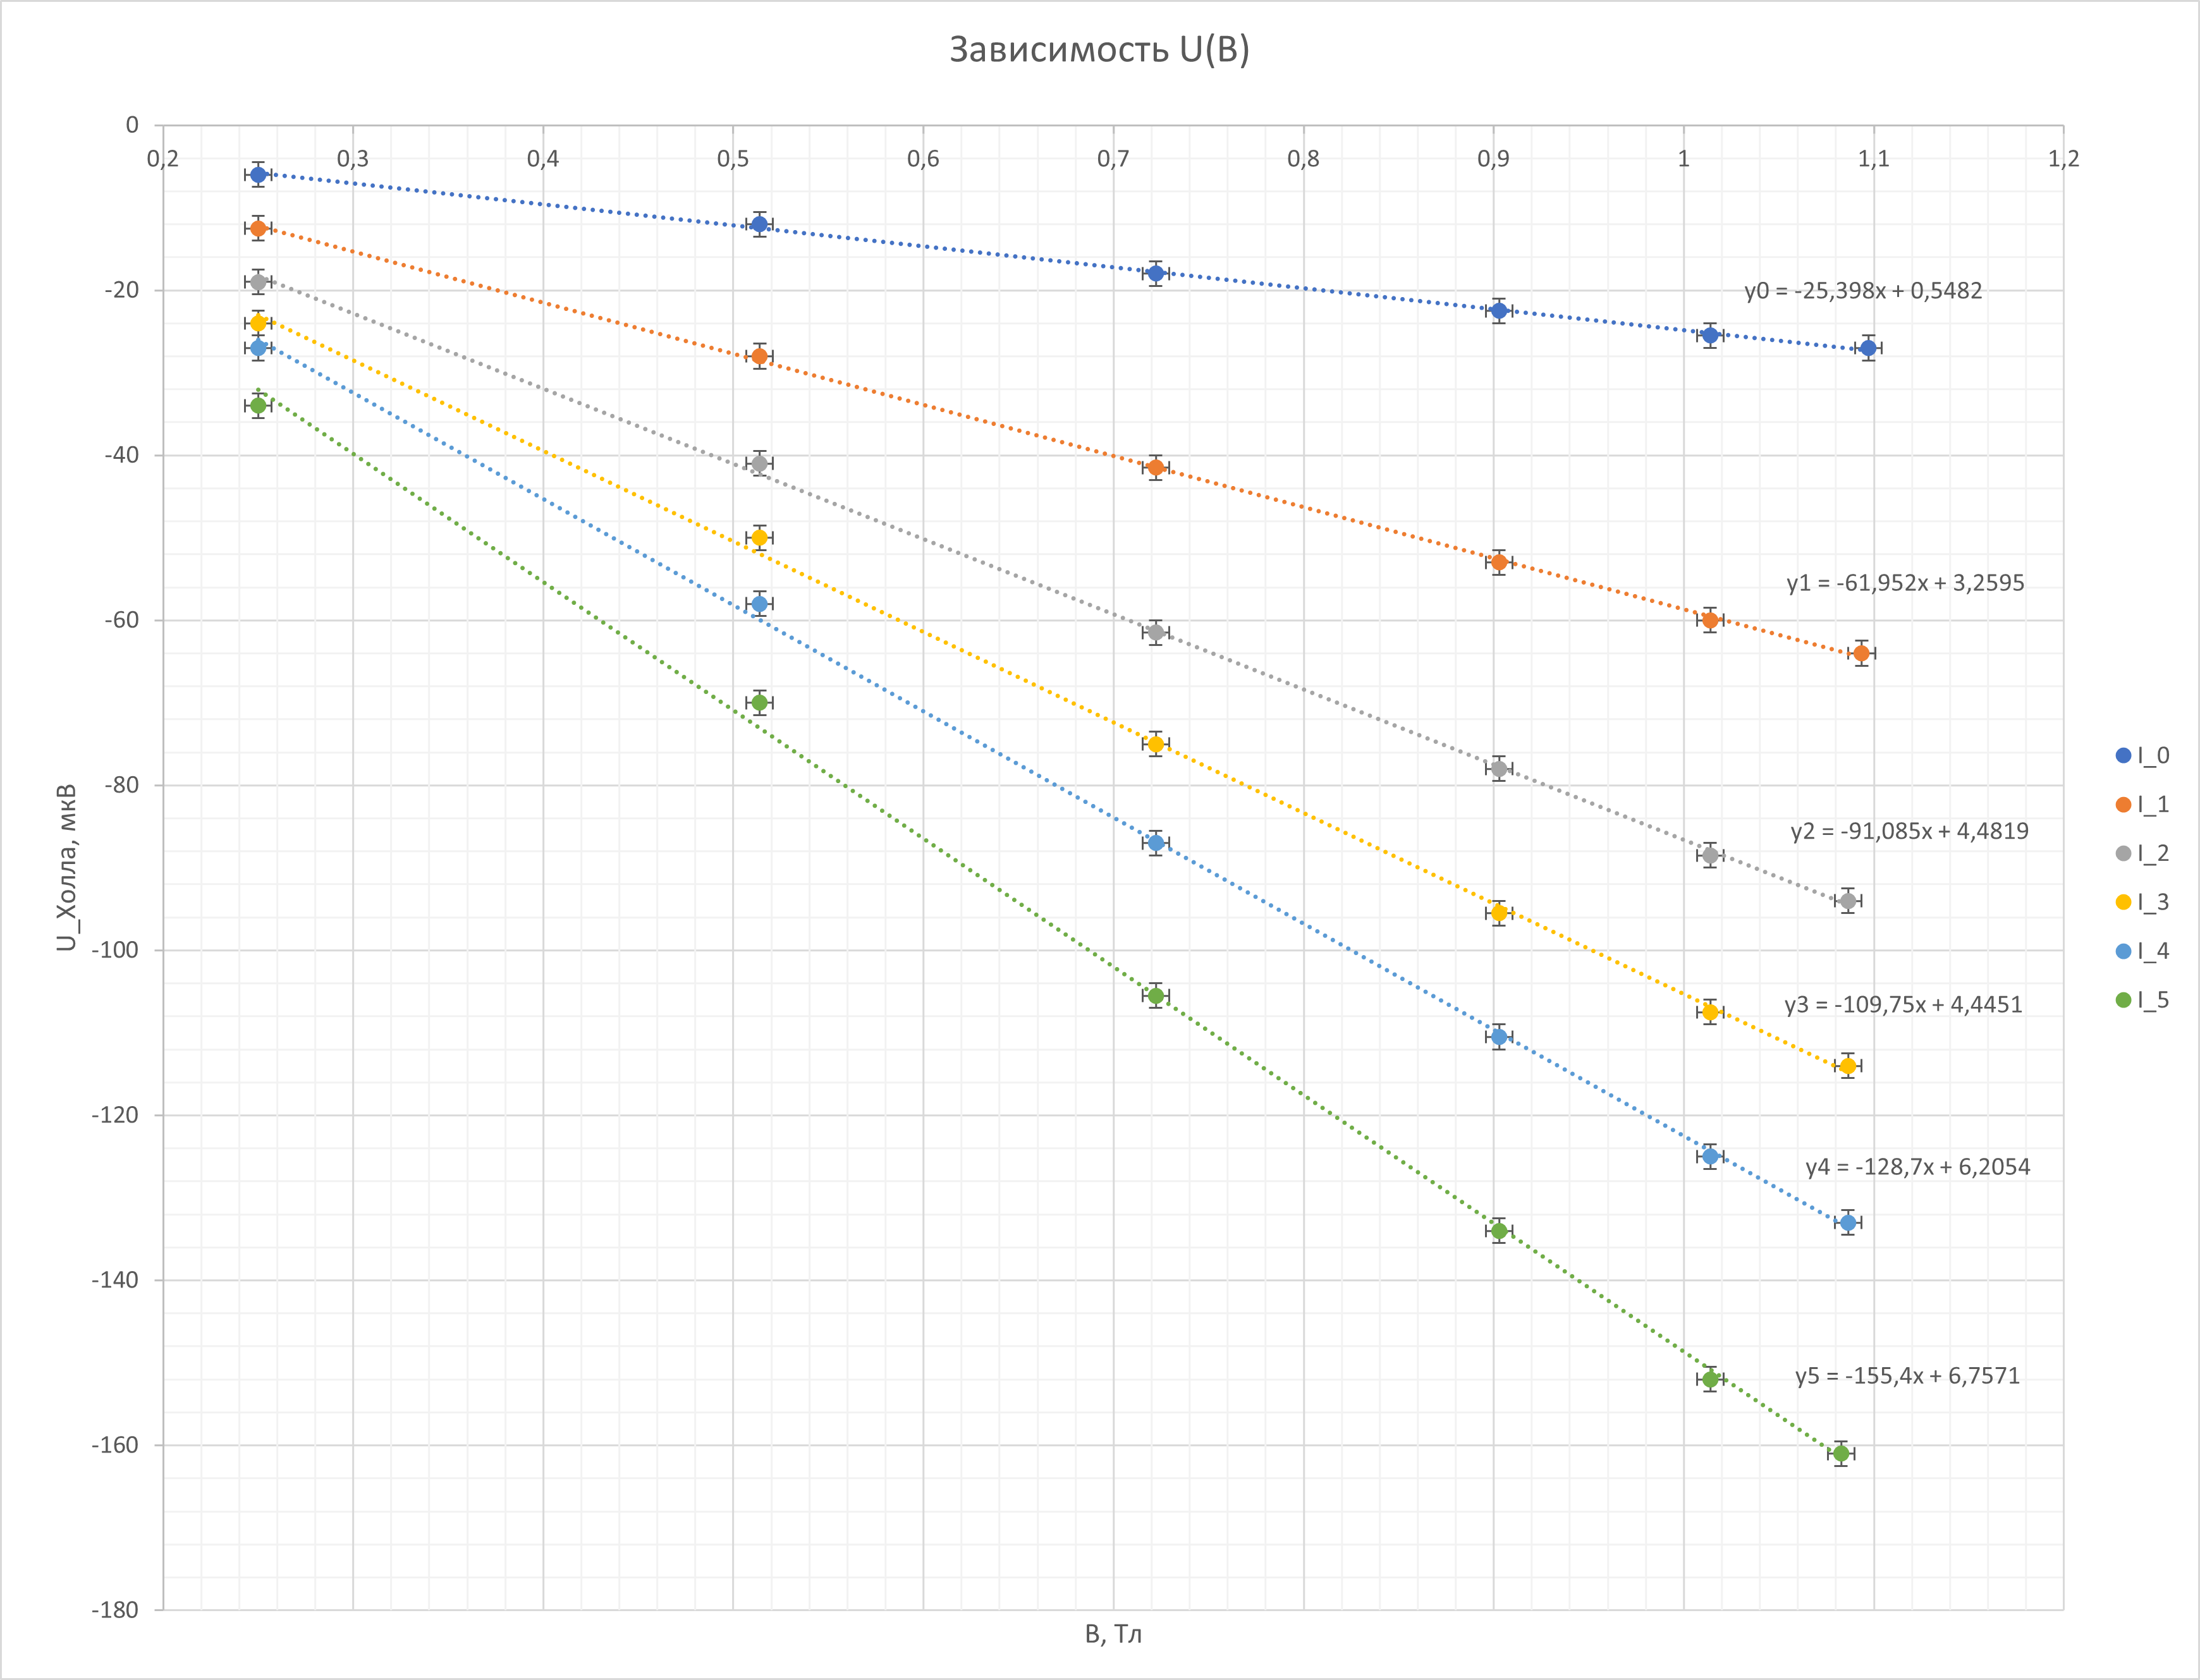
\includegraphics[width = \textwidth]{Gr2}
		\caption{Зависимость $U_{\text{{Холл}}} = f(B)$}
	\end{figure}
	
	Запишем полученные коэффициенты $\frac{dU}{dB}$ в таблицу.
	
	\begin{table}[h]
		\centering
		\begin{tabular}{|c|c|c|c|c|c|c|}
			\hline
			$I_{\text{обр}}$, mA & 0.14 & 0.34 & 0.5 & 0.6 & 0.7 & 0.85 \\ \hline
			$k, \frac{\text{мкВ}}{\text{Тл}}$ & -25.40 & -61.95 & -91.08 & -109.75 & -128.70 & -155.40 \\ \hline
			$\sigma_k$ & 0.51 & 0.68 & 1.21 & 1.80 & 1.71 & 1.73 \\ \hline 
		\end{tabular}
		\caption{Значения коэффициента $\frac{dU}{dB}$ при различных значениях $I_{\text{обр}}$}
	\end{table}
	\newpage
	3) Также определим знак носителей в образце. Узнаем направление тока в образце и в электромагните, с помощью последнего определим направление магнитного поля. Из картинки видно, что носители заряда в экспериментальном проводнике --- электроны.
	
	\begin{figure}
		\centering
		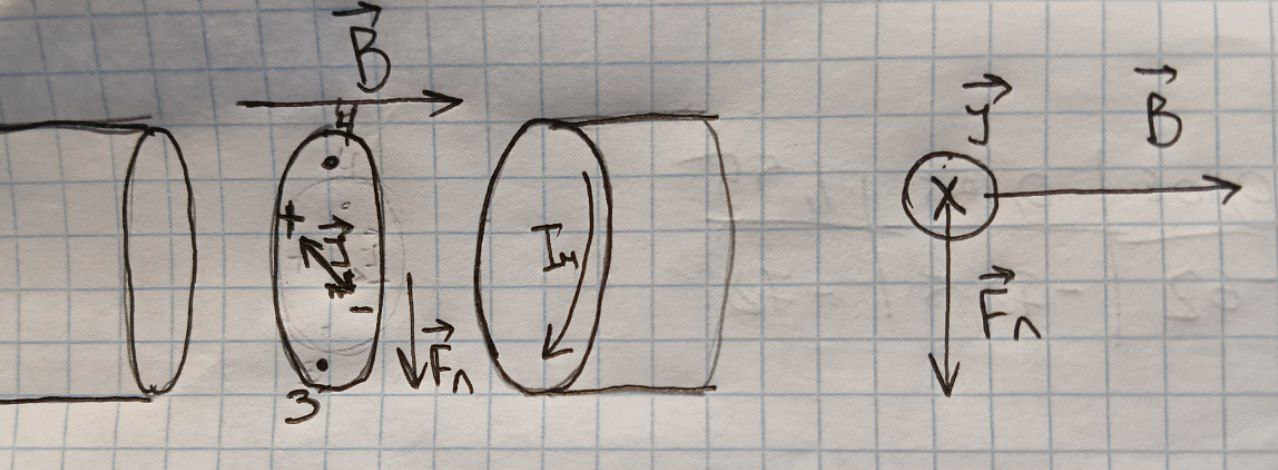
\includegraphics[width=0.8\textwidth]{2}
		\caption{Определение носителей заряда}
	\end{figure}
		
	
	4) Рассчитаем значение параметра $R_H$. Для этого построим график $k = f(I)$ и найдем его наклон.
	
	\begin{figure}[h!]
		\centering
		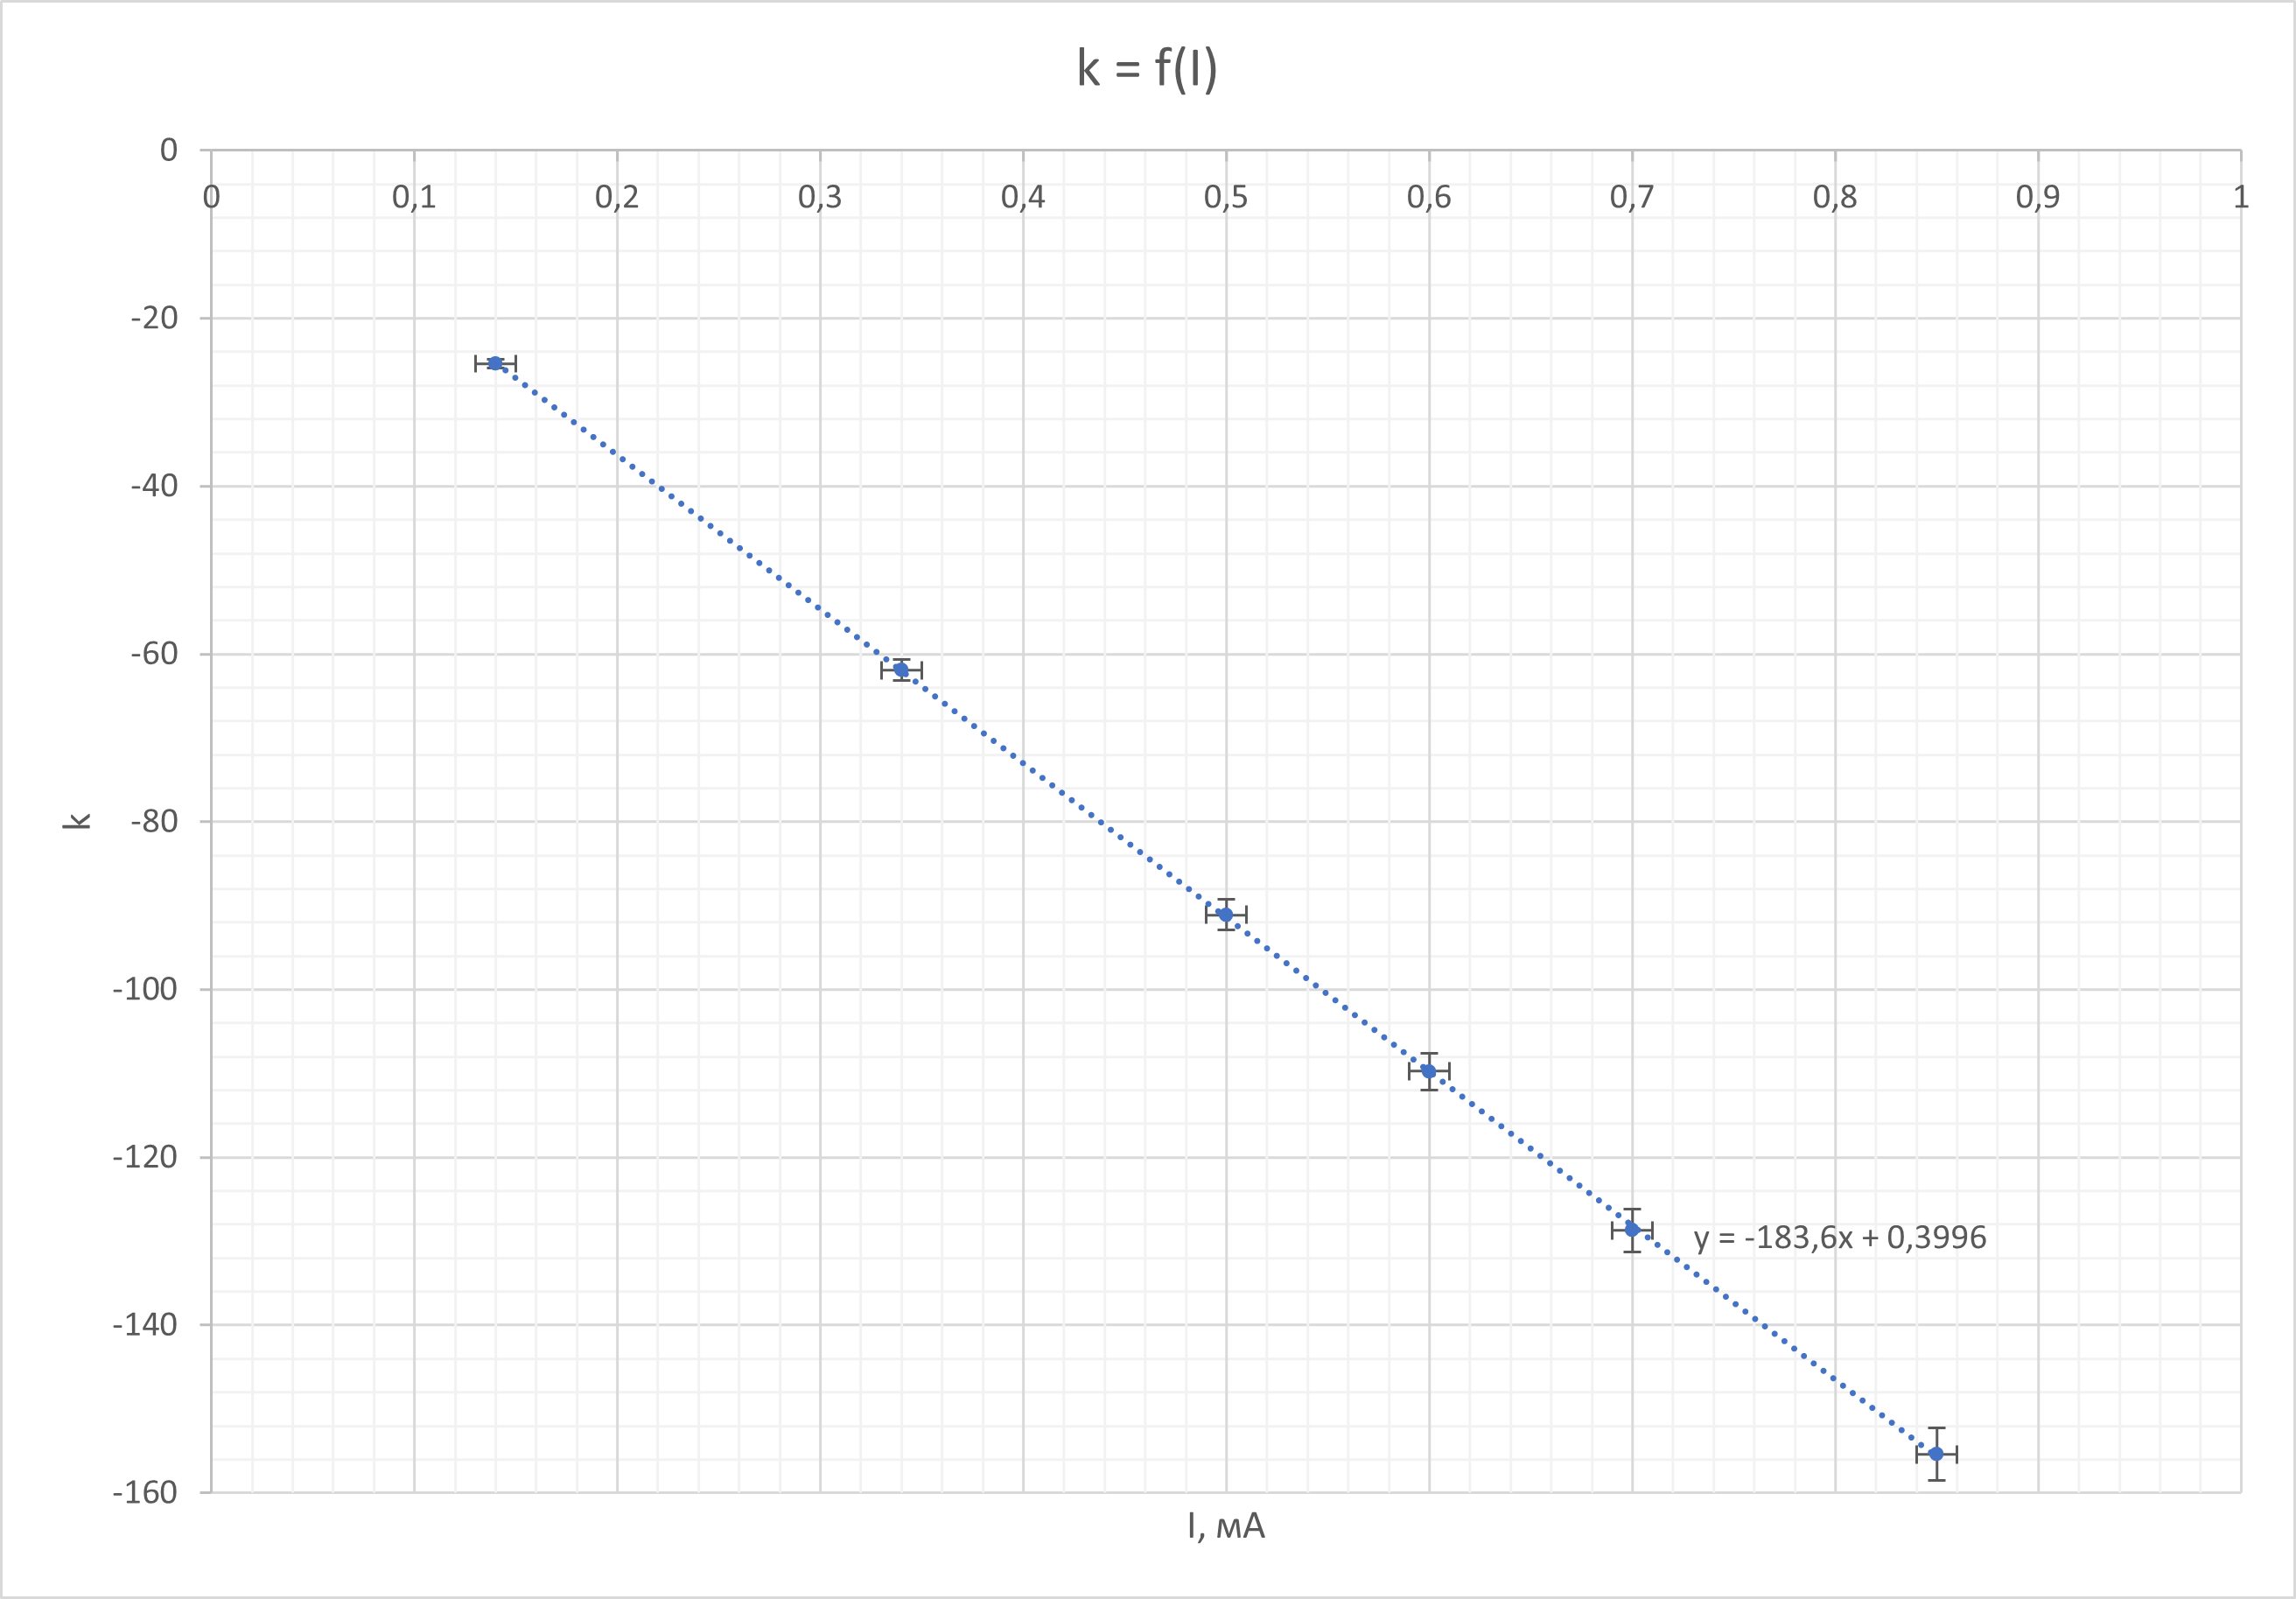
\includegraphics[width=\textwidth]{Gr3}
		\caption{Зависимость $k = f(I)$}
	\end{figure}
	
	\[R_H = h \cdot \frac{dU/dB}{I} = h \cdot \frac{k}{I} = (-403,9 \pm 13,7) \ \frac{\text{см}^3}{\text{Кл}} \ (\varepsilon = 3.4\%)\]
	где $h = 2,2$ мм --- толщина образца.
	
	Значение отрицательное, так как носители заряда в нашем случае --- электроны. Теперь рассчитаем концентрацию носителей заряда:
	\[R_H = \frac{1}{nq} \rightarrow n = \frac{1}{qR_H} = (1.55 \pm 0.05) \cdot 10^{16} \ \ \text{см}^{-3}\]
	
	5) При токе $I = 1,00 \pm 0,01~\text{мА}$ измеряем падение напряжения между концами 3 и 5: $U_{35} = 1,73 \pm 0,01~\text{мВ} $. Характеристики образца: $L_{35} = 3~\text{мм}, a = 2.2~\text{мм}, l = 2.5~\text{мм}$.
	
	Считаем удельную проводимость и удельное сопротивление:
	\[\sigma = \frac{IL_{35}}{U_{35}al} = 315.3 \pm 3.5 \ (\text{Ом}\cdot\text{м})^{-1} \approx  3.15 \ (\text{Ом}\cdot\text{см})^{-1}\]
	\[\rho = \frac{1}{\sigma} = (3.17 \pm 0.03) \cdot 10^{-3} \ \text{Ом}\cdot\text{м} \approx 0.32 \ \text{Ом}\cdot\text{cм}  \]
	
	Вычислим подвижность носителей заряда:
	\[b = \frac{\sigma}{en} = (1.27 \pm 0.05)  \cdot 10^3 \frac{\text{см}^2}{\text{В}\cdot \text{с}} \ (\varepsilon = 3.6\%)\]
	
	\section*{Результаты и выводы}
	
	В данной лабораторной работе были исследованы эффект Холла на полупроводнике из легированного германия и свойства самого полупроводника. Вот все основные результаты: 
	
	\begin{itemize}
		\item $R_H = (-403,9 \pm 13,7) \ \frac{\text{см}^3}{\text{Кл}} \ (\varepsilon = 3.4\%) $
		\item Носителями заряда в экспериментальном проводнике являются электроны
		\item Концентрация носителей заряда $n = (1.55 \pm 0.05) \cdot 10^{16} \ \ \text{см}^{-3} \ (\varepsilon = 3.4\%) $
		\item Проводимость полупроводника: $\sigma = 315.3 \pm 3.5 \ (\text{Ом}\cdot\text{м})^{-1} \ (\varepsilon = 1.1\%)  $
		\item Подвижность носителей заряда $b = (1.27 \pm 0.05)  \cdot 10^3 \ \frac{\text{см}^2}{\text{В}\cdot \text{с}} \ (\varepsilon = 3.6\%) $
	\end{itemize}
	С табличными значениями результаты практически не сходятся, вероятно из-за неизвестного количества примесей в образце полупроводника.
\end{document} 